\documentclass[aspectratio=169, 11pt]{beamer}

\usetheme{Madrid}
\usecolortheme{seahorse}
\setbeamertemplate{navigation symbols}{}
\setbeamertemplate{footline}[frame number]
\setbeamertemplate{itemize items}[circle]

\usepackage{amsmath}
\usepackage{amssymb}
\usepackage{booktabs}
\usepackage{pifont}
\usepackage{tikz}
\usetikzlibrary{arrows.meta, positioning, calc, decorations.pathreplacing, shapes.geometric, fit}

% Custom colors
\definecolor{cblue}{HTML}{2E86C1}
\definecolor{cred}{HTML}{E74C3C}
\definecolor{cgreen}{HTML}{27AE60}
\definecolor{cpurple}{HTML}{8E44AD}
\definecolor{corange}{HTML}{E67E22}
\definecolor{cgray}{HTML}{7F8C8D}
\definecolor{lightblue}{HTML}{D6EAF8}
\definecolor{lightred}{HTML}{FADBD8}
\definecolor{lightgreen}{HTML}{D5F5E3}
\definecolor{lightpurple}{HTML}{E8DAEF}
\definecolor{lightyellow}{HTML}{FEF9E7}
\definecolor{lightorange}{HTML}{FDEBD0}
\definecolor{lightgray}{HTML}{EAECEE}
\definecolor{darkblue}{HTML}{1A5276}

\title{PixelCNN \& Its Improvements}
\subtitle{Understanding Autoregressive Image Generation with Masked Convolutions}
\author{Pan Changxun \\ 2024011323}
\date{Deep Learning, Spring 2026}

\begin{document}

% ============================================================
% TITLE
% ============================================================
\begin{frame}
\titlepage
\end{frame}

% ============================================================
% OUTLINE
% ============================================================
\begin{frame}{Outline}
\tableofcontents
\end{frame}

% ============================================================
\section{Background: Autoregressive Image Generation}
% ============================================================

\begin{frame}{Autoregressive Factorization}
\begin{columns}[c]
\column{0.55\textwidth}
Model the joint distribution of all pixels by the \textbf{chain rule}:
\[
  \boxed{p(\mathbf{x}) = \prod_{i=1}^{n^2} p(x_i \mid x_1, \ldots, x_{i-1})}
\]

\vspace{0.3cm}
Key design choices:
\begin{itemize}
    \item \textbf{Ordering}: raster scan (left-to-right, top-to-bottom)
    \item \textbf{Conditional model}: a neural network
    \item \textbf{Challenge}: how to enforce that $p(x_i | \cdot)$ only depends on \emph{previous} pixels?
\end{itemize}

\column{0.42\textwidth}
\centering
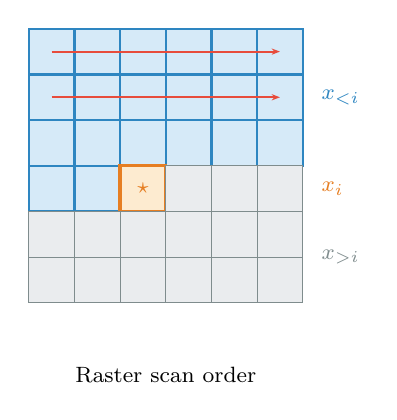
\begin{tikzpicture}[scale=0.58]
  % Draw grid
  \foreach \r in {0,...,5}{
    \foreach \c in {0,...,5}{
      \pgfmathtruncatemacro{\idx}{\r*6+\c}
      \ifnum\idx<20
        \fill[lightblue, draw=cblue, thick] (\c, -\r) rectangle ++(1,-1);
      \else
        \ifnum\idx=20
          \fill[lightorange, draw=corange, very thick] (\c, -\r) rectangle ++(1,-1);
          \node[font=\footnotesize\bfseries, corange] at (\c+0.5, -\r-0.5) {$\star$};
        \else
          \fill[lightgray, draw=cgray] (\c, -\r) rectangle ++(1,-1);
        \fi
      \fi
    }
  }
  % Arrow showing raster order
  \draw[-{Stealth[length=3pt]}, cred, thick] (0.5,-0.5) -- (1.5,-0.5) -- (2.5,-0.5) -- (3.5,-0.5) -- (4.5,-0.5) -- (5.5,-0.5);
  \draw[-{Stealth[length=3pt]}, cred, thick] (0.5,-1.5) -- (1.5,-1.5) -- (2.5,-1.5) -- (3.5,-1.5) -- (4.5,-1.5) -- (5.5,-1.5);

  % Labels
  \node[below, font=\footnotesize] at (3, -7.2) {Raster scan order};
  \node[right, font=\footnotesize, cblue] at (6.2, -1.5) {$x_{<i}$};
  \node[right, font=\footnotesize, corange] at (6.2, -3.5) {$x_i$};
  \node[right, font=\footnotesize, cgray] at (6.2, -5) {$x_{>i}$};
\end{tikzpicture}
\end{columns}
\end{frame}

% ============================================================
\section{PixelCNN: Masked Convolutions}
% ============================================================

\begin{frame}{PixelCNN: Core Idea}
\begin{columns}[c]
\column{0.55\textwidth}
\textbf{Insight}: Use \alert{masked convolution kernels} so that each output pixel only depends on previous pixels in the raster scan order.

\vspace{0.4cm}
Standard convolution:
\[
  y_{r,c} = \sum_{i,j} w_{i,j} \cdot x_{r+i, c+j}
\]

Masked convolution:
\[
  \boxed{y_{r,c} = \sum_{i,j} \underbrace{m_{i,j}}_{\text{mask}} \cdot w_{i,j} \cdot x_{r+i, c+j}}
\]

The mask $m$ zeroes out weights that would access \emph{future} pixels.

\column{0.42\textwidth}
\centering
\textbf{Standard Conv Kernel}\\[0.3cm]
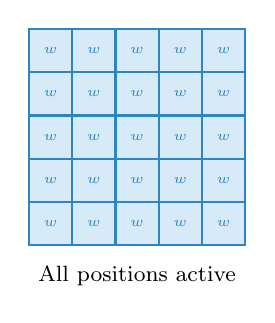
\begin{tikzpicture}[scale=0.55]
  \foreach \r in {0,...,4}{
    \foreach \c in {0,...,4}{
      \fill[lightblue, draw=cblue, thick] (\c, -\r) rectangle ++(1,-1);
      \node[font=\tiny, cblue] at (\c+0.5, -\r-0.5) {$w$};
    }
  }
  \node[font=\footnotesize] at (2.5, -5.7) {All positions active};
\end{tikzpicture}

\vspace{0.3cm}
$\downarrow$ Apply mask $m$ $\downarrow$

\vspace{0.3cm}
\textbf{Masked Conv Kernel}\\[0.3cm]
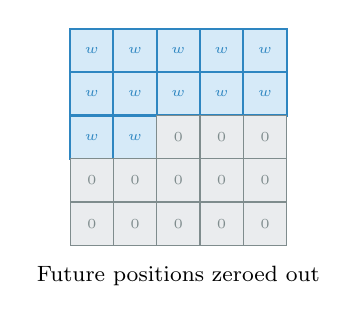
\begin{tikzpicture}[scale=0.55]
  \foreach \r in {0,...,4}{
    \foreach \c in {0,...,4}{
      \pgfmathtruncatemacro{\rmid}{2}
      \ifnum\r<\rmid
        \fill[lightblue, draw=cblue, thick] (\c, -\r) rectangle ++(1,-1);
        \node[font=\tiny, cblue] at (\c+0.5, -\r-0.5) {$w$};
      \else
        \ifnum\r=\rmid
          \ifnum\c<\rmid
            \fill[lightblue, draw=cblue, thick] (\c, -\r) rectangle ++(1,-1);
            \node[font=\tiny, cblue] at (\c+0.5, -\r-0.5) {$w$};
          \else
            \fill[lightgray, draw=cgray] (\c, -\r) rectangle ++(1,-1);
            \node[font=\tiny, cgray] at (\c+0.5, -\r-0.5) {$0$};
          \fi
        \else
          \fill[lightgray, draw=cgray] (\c, -\r) rectangle ++(1,-1);
          \node[font=\tiny, cgray] at (\c+0.5, -\r-0.5) {$0$};
        \fi
      \fi
    }
  }
  \node[font=\footnotesize] at (2.5, -5.7) {Future positions zeroed out};
\end{tikzpicture}
\end{columns}
\end{frame}

% ============================================================
\begin{frame}{The $5 \times 5$ Mask in Detail}
\begin{columns}[c]
\column{0.45\textwidth}
\centering
\textbf{Mask $m$ (from the assignment)}\\[0.4cm]
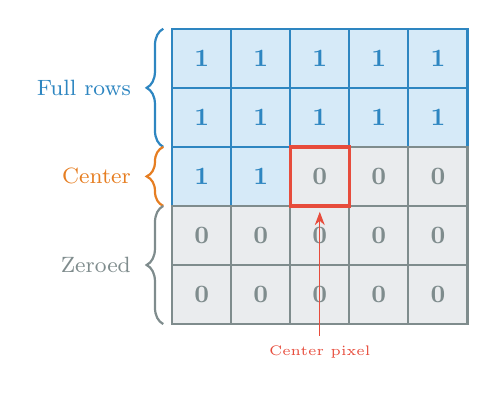
\begin{tikzpicture}[scale=0.75]
  % mask values
  \foreach \r/\vals in {0/{1,1,1,1,1}, 1/{1,1,1,1,1}, 2/{1,1,0,0,0}, 3/{0,0,0,0,0}, 4/{0,0,0,0,0}}{
    \foreach \c/\v in {0/1, 1/1, 2/1, 3/1, 4/1}{
      % extract value
      \pgfmathtruncatemacro{\rmid}{2}
      \pgfmathtruncatemacro{\isactive}{0}
      \ifnum\r<\rmid
        \pgfmathtruncatemacro{\isactive}{1}
      \fi
      \ifnum\r=\rmid
        \ifnum\c<\rmid
          \pgfmathtruncatemacro{\isactive}{1}
        \fi
      \fi
      \ifnum\isactive=1
        \fill[lightblue, draw=cblue, thick] (\c, -\r) rectangle ++(1,-1);
        \node[font=\small\bfseries, cblue] at (\c+0.5, -\r-0.5) {1};
      \else
        \fill[lightgray, draw=cgray, thick] (\c, -\r) rectangle ++(1,-1);
        \node[font=\small\bfseries, cgray] at (\c+0.5, -\r-0.5) {0};
      \fi
    }
  }
  % Annotations
  \draw[decorate, decoration={brace, amplitude=6pt, mirror}, cblue, thick]
    (-0.15, 0) -- (-0.15, -2) node[midway, left=8pt, font=\footnotesize, cblue] {Full rows};
  \draw[decorate, decoration={brace, amplitude=6pt, mirror}, corange, thick]
    (-0.15, -2) -- (-0.15, -3) node[midway, left=8pt, font=\footnotesize, corange] {Center};
  \draw[decorate, decoration={brace, amplitude=6pt, mirror}, cgray, thick]
    (-0.15, -3) -- (-0.15, -5) node[midway, left=8pt, font=\footnotesize, cgray] {Zeroed};
  % Center pixel
  \draw[cred, very thick] (2, -2) rectangle ++(1,-1);
  \node[font=\tiny, cred, below] at (2.5, -5.2) {Center pixel};
  \draw[-{Stealth}, cred] (2.5, -5.2) -- (2.5, -3.1);
\end{tikzpicture}

\column{0.52\textwidth}
Three distinct regions:

\vspace{0.3cm}
\begin{enumerate}
    \item \textcolor{cblue}{\textbf{Upper rows}} (rows 0--1): \\
    All 5 columns = \textbf{1} \\
    $\Rightarrow$ See \emph{full width} above

    \vspace{0.2cm}
    \item \textcolor{corange}{\textbf{Center row}} (row 2): \\
    Only left 2 columns = \textbf{1} \\
    $\Rightarrow$ See only \emph{left neighbors}

    \vspace{0.2cm}
    \item \textcolor{cgray}{\textbf{Lower rows}} (rows 3--4): \\
    All columns = \textbf{0} \\
    $\Rightarrow$ \emph{Completely invisible}
\end{enumerate}

\vspace{0.3cm}
\begin{alertblock}{Key Asymmetry}
Upper rows: left \textbf{and} right visible.\\
Center row: \textbf{only left} visible.\\
This asymmetry causes the sawtooth!
\end{alertblock}
\end{columns}
\end{frame}

% ============================================================
\begin{frame}{Type A vs Type B Masks}
\begin{columns}[c]
\column{0.45\textwidth}
\centering
\textbf{Type A Mask (1st layer)}\\[0.3cm]
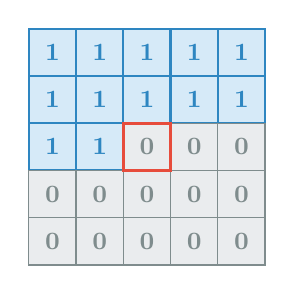
\begin{tikzpicture}[scale=0.6]
  \foreach \r in {0,...,4}{
    \foreach \c in {0,...,4}{
      \pgfmathtruncatemacro{\isactive}{0}
      \ifnum\r<2 \pgfmathtruncatemacro{\isactive}{1} \fi
      \ifnum\r=2
        \ifnum\c<2 \pgfmathtruncatemacro{\isactive}{1} \fi
      \fi
      \ifnum\isactive=1
        \fill[lightblue, draw=cblue, thick] (\c, -\r) rectangle ++(1,-1);
        \node[font=\small\bfseries, cblue] at (\c+0.5, -\r-0.5) {1};
      \else
        \fill[lightgray, draw=cgray] (\c, -\r) rectangle ++(1,-1);
        \node[font=\small\bfseries, cgray] at (\c+0.5, -\r-0.5) {0};
      \fi
    }
  }
  \draw[cred, very thick] (2,-2) rectangle ++(1,-1);
\end{tikzpicture}

\vspace{0.2cm}
Center pixel is \textbf{excluded} (0).\\
Used in the \textbf{first} layer only ---\\
the pixel cannot see \emph{itself}.

\column{0.45\textwidth}
\centering
\textbf{Type B Mask (layers 2+)}\\[0.3cm]
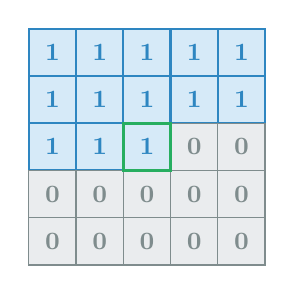
\begin{tikzpicture}[scale=0.6]
  \foreach \r in {0,...,4}{
    \foreach \c in {0,...,4}{
      \pgfmathtruncatemacro{\isactive}{0}
      \ifnum\r<2 \pgfmathtruncatemacro{\isactive}{1} \fi
      \ifnum\r=2
        \ifnum\c<3 \pgfmathtruncatemacro{\isactive}{1} \fi
      \fi
      \ifnum\isactive=1
        \fill[lightblue, draw=cblue, thick] (\c, -\r) rectangle ++(1,-1);
        \node[font=\small\bfseries, cblue] at (\c+0.5, -\r-0.5) {1};
      \else
        \fill[lightgray, draw=cgray] (\c, -\r) rectangle ++(1,-1);
        \node[font=\small\bfseries, cgray] at (\c+0.5, -\r-0.5) {0};
      \fi
    }
  }
  \draw[cgreen, very thick] (2,-2) rectangle ++(1,-1);
\end{tikzpicture}

\vspace{0.2cm}
Center pixel is \textbf{included} (1).\\
Used in \textbf{subsequent} layers ---\\
features at the same position carry\\
information from prior pixels only.
\end{columns}

\vspace{0.3cm}
\centering
\textit{Both masks preserve the autoregressive property: $x_i$ never depends on $x_j$ for $j \geq i$ in the input.}
\end{frame}

% ============================================================
\section{Receptive Field \& Sawtooth Pattern}
% ============================================================

\begin{frame}{Receptive Field After 1 Layer ($3\times 3$ kernel)}
\begin{columns}[c]
\column{0.5\textwidth}
\centering
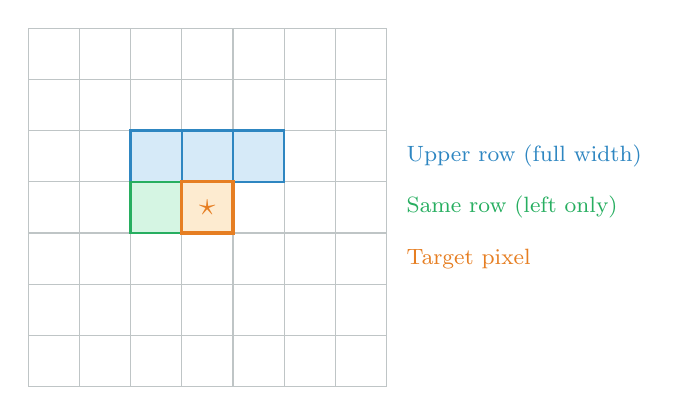
\begin{tikzpicture}[scale=0.65]
  % Draw 7x7 grid
  \foreach \r in {0,...,6}{
    \foreach \c in {0,...,6}{
      \fill[white, draw=cgray!50] (\c, -\r) rectangle ++(1,-1);
    }
  }
  % RF after 1 layer: row 2 cols 2-4, row 3 col 2
  % Target at (3,3)
  % Row above (r-1=2): c-1=2, c=3, c+1=4
  \fill[lightblue, draw=cblue, thick] (2, -2) rectangle ++(1,-1);
  \fill[lightblue, draw=cblue, thick] (3, -2) rectangle ++(1,-1);
  \fill[lightblue, draw=cblue, thick] (4, -2) rectangle ++(1,-1);
  % Same row: c-1=2
  \fill[lightgreen, draw=cgreen, thick] (2, -3) rectangle ++(1,-1);
  % Target
  \fill[lightorange, draw=corange, very thick] (3, -3) rectangle ++(1,-1);
  \node[font=\large\bfseries, corange] at (3.5, -3.5) {$\star$};

  % Labels
  \node[font=\footnotesize, cblue, right] at (7.2, -2.5) {Upper row (full width)};
  \node[font=\footnotesize, cgreen, right] at (7.2, -3.5) {Same row (left only)};
  \node[font=\footnotesize, corange, right] at (7.2, -4.5) {Target pixel};
\end{tikzpicture}

\column{0.47\textwidth}
With a $3\times 3$ masked kernel ($h=1$):

\vspace{0.3cm}
\begin{itemize}
    \item \textcolor{cblue}{\textbf{Row above}}: sees columns $c{-}1, c, c{+}1$ \\
    (3 pixels, full width)
    \item \textcolor{cgreen}{\textbf{Same row}}: sees only $c{-}1$ \\
    (1 pixel, left only)
    \item \textcolor{cgray}{\textbf{Below}}: nothing
\end{itemize}

\vspace{0.3cm}
RF size: \textbf{4 pixels}.\\
Right boundary: $c{+}1$ above, $c{-}1$ on same row.
\end{columns}
\end{frame}

% ============================================================
\begin{frame}{Receptive Field Growth: 1, 2, 3 Layers}
\begin{columns}[t]
\column{0.32\textwidth}
\centering
\textbf{1 Layer}\\[0.3cm]
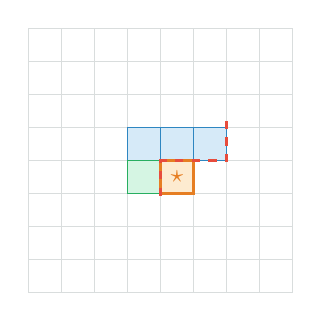
\begin{tikzpicture}[scale=0.42]
  \foreach \r in {0,...,7}{
    \foreach \c in {0,...,7}{
      \fill[white, draw=cgray!30] (\c, -\r) rectangle ++(1,-1);
    }
  }
  % Layer 1 RF at target (4,4) with 3x3 kernel
  % Row 3: cols 3,4,5
  \fill[lightblue, draw=cblue] (3,-3) rectangle ++(1,-1);
  \fill[lightblue, draw=cblue] (4,-3) rectangle ++(1,-1);
  \fill[lightblue, draw=cblue] (5,-3) rectangle ++(1,-1);
  % Row 4: col 3
  \fill[lightgreen, draw=cgreen] (3,-4) rectangle ++(1,-1);
  % Target
  \fill[lightorange, draw=corange, thick] (4,-4) rectangle ++(1,-1);
  \node[font=\small\bfseries, corange] at (4.5,-4.5) {$\star$};

  % Right boundary line
  \draw[cred, very thick, dashed] (6, -2.8) -- (6, -4) -- (4, -4) -- (4, -5.2);
\end{tikzpicture}

\column{0.32\textwidth}
\centering
\textbf{2 Layers}\\[0.3cm]
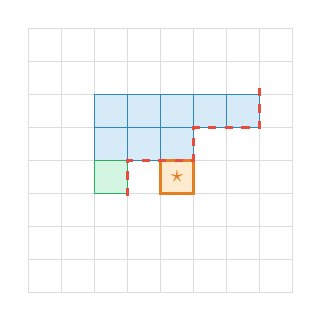
\begin{tikzpicture}[scale=0.42]
  \foreach \r in {0,...,7}{
    \foreach \c in {0,...,7}{
      \fill[white, draw=cgray!30] (\c, -\r) rectangle ++(1,-1);
    }
  }
  % Layer 2 RF at target (4,4)
  % Row 2: cols 2,3,4,5,6
  \fill[lightblue, draw=cblue] (2,-2) rectangle ++(1,-1);
  \fill[lightblue, draw=cblue] (3,-2) rectangle ++(1,-1);
  \fill[lightblue, draw=cblue] (4,-2) rectangle ++(1,-1);
  \fill[lightblue, draw=cblue] (5,-2) rectangle ++(1,-1);
  \fill[lightblue, draw=cblue] (6,-2) rectangle ++(1,-1);
  % Row 3: cols 2,3,4
  \fill[lightblue, draw=cblue] (2,-3) rectangle ++(1,-1);
  \fill[lightblue, draw=cblue] (3,-3) rectangle ++(1,-1);
  \fill[lightblue, draw=cblue] (4,-3) rectangle ++(1,-1);
  % Row 4: col 2
  \fill[lightgreen, draw=cgreen] (2,-4) rectangle ++(1,-1);
  % Target
  \fill[lightorange, draw=corange, thick] (4,-4) rectangle ++(1,-1);
  \node[font=\small\bfseries, corange] at (4.5,-4.5) {$\star$};

  % Right boundary
  \draw[cred, very thick, dashed] (7, -1.8) -- (7, -3) -- (5, -3) -- (5, -4) -- (3, -4) -- (3, -5.2);
\end{tikzpicture}

\column{0.32\textwidth}
\centering
\textbf{3 Layers}\\[0.3cm]
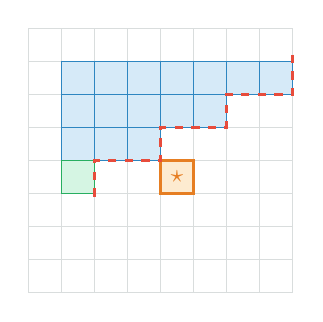
\begin{tikzpicture}[scale=0.42]
  \foreach \r in {0,...,7}{
    \foreach \c in {0,...,7}{
      \fill[white, draw=cgray!30] (\c, -\r) rectangle ++(1,-1);
    }
  }
  % Layer 3 RF at target (4,4)
  % Row 1: cols 1..7
  \fill[lightblue, draw=cblue] (1,-1) rectangle ++(1,-1);
  \fill[lightblue, draw=cblue] (2,-1) rectangle ++(1,-1);
  \fill[lightblue, draw=cblue] (3,-1) rectangle ++(1,-1);
  \fill[lightblue, draw=cblue] (4,-1) rectangle ++(1,-1);
  \fill[lightblue, draw=cblue] (5,-1) rectangle ++(1,-1);
  \fill[lightblue, draw=cblue] (6,-1) rectangle ++(1,-1);
  \fill[lightblue, draw=cblue] (7,-1) rectangle ++(1,-1);
  % Row 2: cols 1..5
  \fill[lightblue, draw=cblue] (1,-2) rectangle ++(1,-1);
  \fill[lightblue, draw=cblue] (2,-2) rectangle ++(1,-1);
  \fill[lightblue, draw=cblue] (3,-2) rectangle ++(1,-1);
  \fill[lightblue, draw=cblue] (4,-2) rectangle ++(1,-1);
  \fill[lightblue, draw=cblue] (5,-2) rectangle ++(1,-1);
  % Row 3: cols 1..3
  \fill[lightblue, draw=cblue] (1,-3) rectangle ++(1,-1);
  \fill[lightblue, draw=cblue] (2,-3) rectangle ++(1,-1);
  \fill[lightblue, draw=cblue] (3,-3) rectangle ++(1,-1);
  % Row 4: col 1
  \fill[lightgreen, draw=cgreen] (1,-4) rectangle ++(1,-1);
  % Target
  \fill[lightorange, draw=corange, thick] (4,-4) rectangle ++(1,-1);
  \node[font=\small\bfseries, corange] at (4.5,-4.5) {$\star$};

  % Right boundary - sawtooth
  \draw[cred, very thick, dashed] (8, -0.8) -- (8, -2) -- (6, -2) -- (6, -3) -- (4, -3) -- (4, -4) -- (2, -4) -- (2, -5.2);
\end{tikzpicture}
\end{columns}

\vspace{0.3cm}
\centering
The \textcolor{cred}{\textbf{red dashed line}} is the right boundary --- it forms a \alert{staircase / sawtooth} shape.\\
Each row going down, the right boundary shifts left. Upper rows expand both ways; current row only expands left.
\end{frame}

% ============================================================
\begin{frame}{The Sawtooth Pattern Explained}
\begin{columns}[c]
\column{0.48\textwidth}
\centering
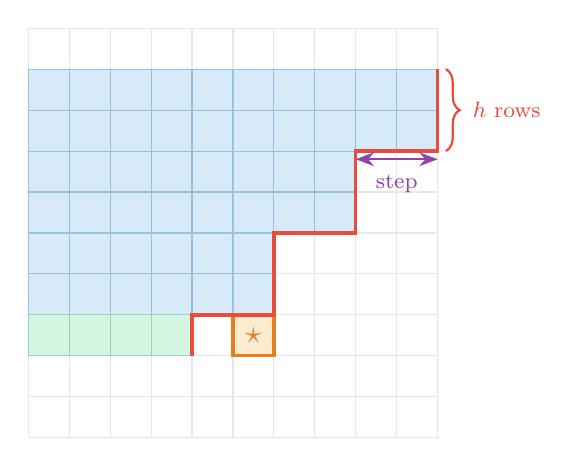
\begin{tikzpicture}[scale=0.52]
  % Draw a large grid 10x10
  \foreach \r in {0,...,9}{
    \foreach \c in {0,...,9}{
      \fill[white, draw=cgray!20] (\c, -\r) rectangle ++(1,-1);
    }
  }

  % Sawtooth RF shape (approximate after several layers, 5x5 kernel)
  % Upper part - wider teeth
  \foreach \c in {0,...,9}{
    \fill[lightblue, draw=cblue!50] (\c, -1) rectangle ++(1,-1);
    \fill[lightblue, draw=cblue!50] (\c, -2) rectangle ++(1,-1);
  }
  \foreach \c in {0,...,7}{
    \fill[lightblue, draw=cblue!50] (\c, -3) rectangle ++(1,-1);
    \fill[lightblue, draw=cblue!50] (\c, -4) rectangle ++(1,-1);
  }
  \foreach \c in {0,...,5}{
    \fill[lightblue, draw=cblue!50] (\c, -5) rectangle ++(1,-1);
    \fill[lightblue, draw=cblue!50] (\c, -6) rectangle ++(1,-1);
  }
  \foreach \c in {0,...,3}{
    \fill[lightgreen, draw=cgreen!50] (\c, -7) rectangle ++(1,-1);
  }

  % Target
  \fill[lightorange, draw=corange, very thick] (5, -7) rectangle ++(1,-1);
  \node[font=\large\bfseries, corange] at (5.5, -7.5) {$\star$};

  % Right boundary - sawtooth with h=2 teeth
  \draw[cred, very thick] (10, -1) -- (10, -3) -- (8, -3) -- (8, -5) -- (6, -5) -- (6, -7) -- (4, -7) -- (4, -8);

  % Annotations
  \draw[decorate, decoration={brace, amplitude=5pt}, cred, thick]
    (10.2, -1) -- (10.2, -3) node[midway, right=6pt, font=\footnotesize, cred] {$h$ rows};
  \draw[{Stealth}-{Stealth}, cpurple, thick] (8, -3.2) -- (10, -3.2) node[midway, below=2pt, font=\footnotesize, cpurple] {step};
\end{tikzpicture}

\column{0.5\textwidth}
For a $5\times 5$ kernel ($h=2$):

\vspace{0.3cm}
\begin{itemize}
    \item The right boundary stays \textbf{flat} for $h=2$ rows (a ``tooth'')
    \item Then it \textbf{drops} by $h$ columns
    \item Repeat: flat $\to$ drop $\to$ flat $\to$ drop
\end{itemize}

\vspace{0.3cm}
\textbf{Why?}
\begin{itemize}
    \item The mask has $h=2$ full rows above center $\Rightarrow$ each layer adds $h$ rows of symmetric expansion
    \item On the center row, only leftward expansion
    \item The periodic ``$h$ flat + step'' pattern creates the sawtooth
\end{itemize}

\vspace{0.3cm}
\begin{block}{Consequence}
The right boundary is a staircase, \emph{not} a smooth diagonal. The upper-right region is never reached.
\end{block}
\end{columns}
\end{frame}

% ============================================================
\section{The Blind Spot Problem}
% ============================================================

\begin{frame}{Ideal RF vs Actual RF: The Blind Spot}
\begin{columns}[c]
\column{0.45\textwidth}
\centering
\textbf{Ideal Receptive Field}\\
(all previous pixels in raster order)\\[0.3cm]
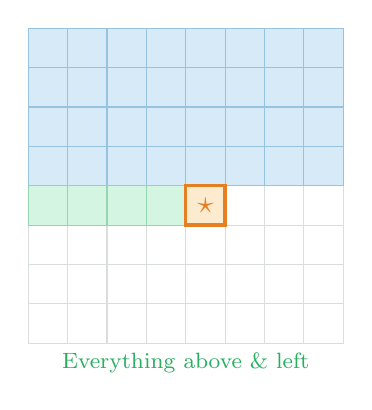
\begin{tikzpicture}[scale=0.5]
  \foreach \r in {0,...,7}{
    \foreach \c in {0,...,7}{
      \fill[white, draw=cgray!30] (\c, -\r) rectangle ++(1,-1);
    }
  }
  % All pixels before (4,4) in raster order
  \foreach \r in {0,...,3}{
    \foreach \c in {0,...,7}{
      \fill[lightblue, draw=cblue!50] (\c, -\r) rectangle ++(1,-1);
    }
  }
  % Row 4: cols 0..3
  \foreach \c in {0,...,3}{
    \fill[lightgreen, draw=cgreen!50] (\c, -4) rectangle ++(1,-1);
  }
  % Target
  \fill[lightorange, draw=corange, very thick] (4, -4) rectangle ++(1,-1);
  \node[font=\large\bfseries, corange] at (4.5, -4.5) {$\star$};

  \node[font=\footnotesize, cgreen] at (4, -8.5) {Everything above \& left};
\end{tikzpicture}

\column{0.45\textwidth}
\centering
\textbf{Actual Receptive Field}\\
(after stacking masked conv layers)\\[0.3cm]
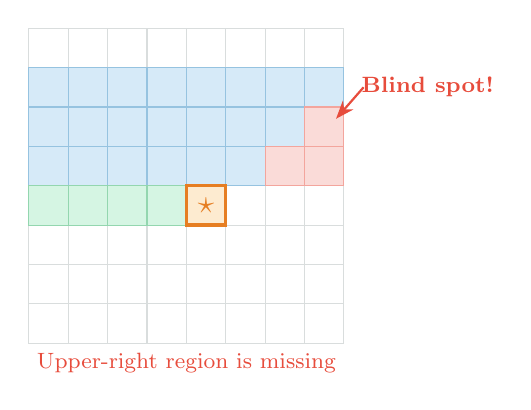
\begin{tikzpicture}[scale=0.5]
  \foreach \r in {0,...,7}{
    \foreach \c in {0,...,7}{
      \fill[white, draw=cgray!30] (\c, -\r) rectangle ++(1,-1);
    }
  }
  % Sawtooth-shaped RF
  \foreach \c in {0,...,7}{
    \fill[lightblue, draw=cblue!50] (\c, -1) rectangle ++(1,-1);
  }
  \foreach \c in {0,...,6}{
    \fill[lightblue, draw=cblue!50] (\c, -2) rectangle ++(1,-1);
  }
  \foreach \c in {0,...,5}{
    \fill[lightblue, draw=cblue!50] (\c, -3) rectangle ++(1,-1);
  }
  \foreach \c in {0,...,3}{
    \fill[lightgreen, draw=cgreen!50] (\c, -4) rectangle ++(1,-1);
  }

  % Blind spot region
  \fill[lightred, draw=cred!50] (7, -2) rectangle ++(1,-1);
  \fill[lightred, draw=cred!50] (6, -3) rectangle ++(1,-1);
  \fill[lightred, draw=cred!50] (7, -3) rectangle ++(1,-1);

  % Target
  \fill[lightorange, draw=corange, very thick] (4, -4) rectangle ++(1,-1);
  \node[font=\large\bfseries, corange] at (4.5, -4.5) {$\star$};

  % Blind spot label
  \draw[-{Stealth}, cred, thick] (8.5, -1.5) -- (7.8, -2.3);
  \node[font=\footnotesize\bfseries, cred, right] at (8.2, -1.5) {Blind spot!};

  \node[font=\footnotesize, cred] at (4, -8.5) {Upper-right region is missing};
\end{tikzpicture}
\end{columns}

\vspace{0.2cm}
\centering
\alert{The blind spot = upper-right pixels that should be visible but are not reachable by stacked masked convolutions.}
\end{frame}

% ============================================================
\begin{frame}{Why Does the Blind Spot Exist?}
\centering
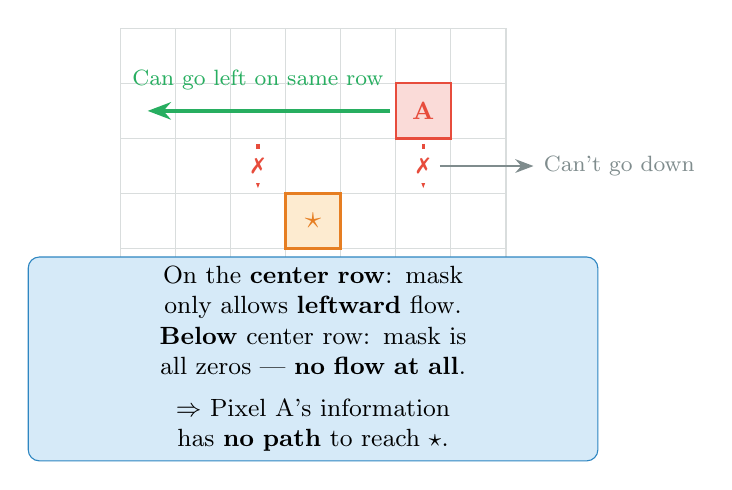
\begin{tikzpicture}[scale=0.7, every node/.style={font=\small}]
  % Grid
  \foreach \r in {0,...,4}{
    \foreach \c in {0,...,6}{
      \fill[white, draw=cgray!30] (\c, -\r) rectangle ++(1,-1);
    }
  }

  % Upper-right pixel
  \fill[lightred, draw=cred, thick] (5, -1) rectangle ++(1,-1);
  \node[font=\small\bfseries, cred] at (5.5, -1.5) {A};

  % Target pixel
  \fill[lightorange, draw=corange, very thick] (3, -3) rectangle ++(1,-1);
  \node[font=\large\bfseries, corange] at (3.5, -3.5) {$\star$};

  % Attempt path 1: A goes right? No!
  \draw[-{Stealth}, cred, very thick, dashed] (5.5, -2.1) -- (5.5, -2.9);
  \node[font=\footnotesize, cred, fill=white] at (5.5, -2.5) {\ding{55}};
  \draw[-{Stealth}, cgray, thick] (5.8, -2.5) -- (7.5, -2.5) node[right, font=\footnotesize] {Can't go down};

  % Attempt path 2: go left on same row? Only if already on the row
  \draw[-{Stealth}, cgreen, very thick] (4.9, -1.5) -- (0.5, -1.5);
  \node[font=\footnotesize, cgreen, above] at (2.5, -1.3) {Can go left on same row};

  % But no downward path
  \draw[-{Stealth}, cred, very thick, dashed] (2.5, -2.1) -- (2.5, -2.9);
  \node[font=\footnotesize, cred, fill=white] at (2.5, -2.5) {\ding{55}};

  % Explanation boxes
  \node[draw=cblue, fill=lightblue, rounded corners, text width=7cm, align=center, font=\small]
    at (3.5, -6) {
      On the \textbf{center row}: mask only allows \textbf{leftward} flow.\\
      \textbf{Below} center row: mask is all zeros --- \textbf{no flow at all}.\\[4pt]
      $\Rightarrow$ Pixel A's information has \textbf{no path} to reach $\star$.
    };
\end{tikzpicture}

\vspace{0.2cm}
The issue: information on row $r{-}k$ at column $c{+}j$ must first travel \emph{down} to row $r$, but the mask blocks all downward propagation except through the upper rows of the next layer's kernel --- which shifts the right boundary left.
\end{frame}

% ============================================================
\section{Solution: Gated PixelCNN}
% ============================================================

\begin{frame}{Key Idea: Split into Two Stacks}
\begin{center}
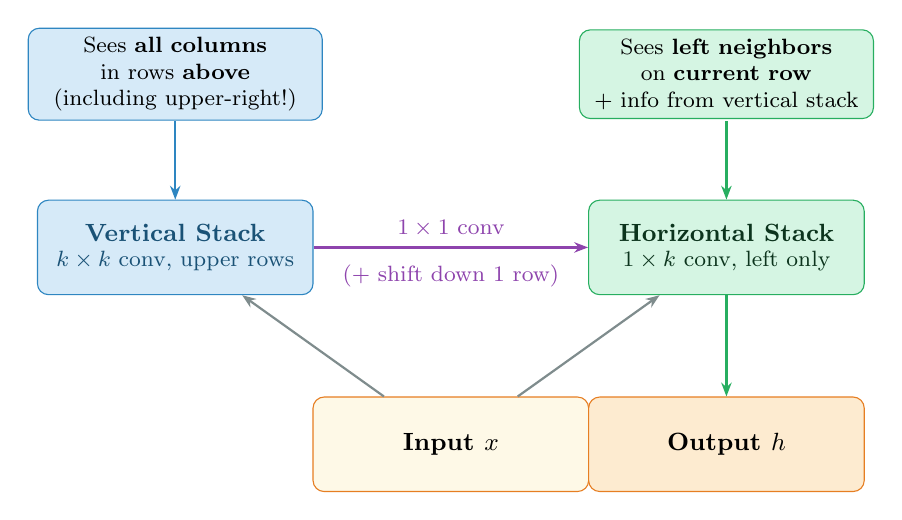
\begin{tikzpicture}[
  box/.style={draw, rounded corners=4pt, minimum width=3.5cm, minimum height=1.2cm, align=center, font=\small\bfseries},
  arr/.style={-{Stealth[length=5pt]}, thick}
]

  % Vertical Stack
  \node[box, fill=lightblue, draw=cblue, text=darkblue] (vs) at (0, 0) {Vertical Stack\\[-2pt]\footnotesize\normalfont $k \times k$ conv, upper rows};

  % Horizontal Stack
  \node[box, fill=lightgreen, draw=cgreen, text=cgreen!30!black] (hs) at (7, 0) {Horizontal Stack\\[-2pt]\footnotesize\normalfont $1 \times k$ conv, left only};

  % 1x1 conv connection
  \draw[arr, cpurple, very thick] (vs) -- (hs) node[midway, above, font=\footnotesize, cpurple] {$1\times 1$ conv};
  \node[font=\footnotesize, cpurple, below] at (3.5, -0.1) {(+ shift down 1 row)};

  % Input
  \node[box, fill=lightyellow, draw=corange] (input) at (3.5, -2.5) {Input $x$};
  \draw[arr, cgray] (input) -- (vs);
  \draw[arr, cgray] (input) -- (hs);

  % Output
  \node[box, fill=lightorange, draw=corange] (output) at (7, -2.5) {Output $h$};
  \draw[arr, cgreen, thick] (hs) -- (output);

  % Labels for what each sees
  \node[draw=cblue, fill=lightblue, rounded corners, font=\footnotesize, text width=3.5cm, align=center]
    at (0, 2.2) {Sees \textbf{all columns}\\in rows \textbf{above}\\(including upper-right!)};
  \draw[arr, cblue] (0, 1.6) -- (vs);

  \node[draw=cgreen, fill=lightgreen, rounded corners, font=\footnotesize, text width=3.5cm, align=center]
    at (7, 2.2) {Sees \textbf{left neighbors}\\on \textbf{current row}\\+ info from vertical stack};
  \draw[arr, cgreen] (7, 1.6) -- (hs);

\end{tikzpicture}
\end{center}

\vspace{0.2cm}
\begin{block}{Core Insight}
Separate ``looking up'' (vertical) from ``looking left'' (horizontal), then \textbf{connect} them. The vertical stack captures the upper-right region that was the blind spot!
\end{block}
\end{frame}

% ============================================================
\begin{frame}{Vertical Stack: See Everything Above}
\begin{columns}[c]
\column{0.45\textwidth}
\centering
\textbf{Vertical Mask} ($5 \times 5$)\\[0.3cm]
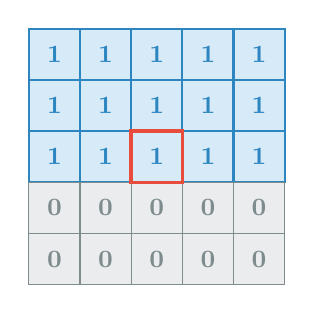
\begin{tikzpicture}[scale=0.65]
  \foreach \r in {0,...,4}{
    \foreach \c in {0,...,4}{
      \pgfmathtruncatemacro{\isactive}{0}
      \ifnum\r<3 \pgfmathtruncatemacro{\isactive}{1} \fi
      \ifnum\isactive=1
        \fill[lightblue, draw=cblue, thick] (\c, -\r) rectangle ++(1,-1);
        \node[font=\small\bfseries, cblue] at (\c+0.5, -\r-0.5) {1};
      \else
        \fill[lightgray, draw=cgray] (\c, -\r) rectangle ++(1,-1);
        \node[font=\small\bfseries, cgray] at (\c+0.5, -\r-0.5) {0};
      \fi
    }
  }
  \draw[cred, very thick] (2,-2) rectangle ++(1,-1);
\end{tikzpicture}

\vspace{0.3cm}
Top 3 rows: \textbf{all} columns active.\\
Center row included, bottom rows zero.

\column{0.5\textwidth}
\textbf{Computation:}
\[
  v = \mathrm{conv}(m_v \cdot w_v, \; x)
\]

\vspace{0.2cm}
\alert{Critical step: shift output down by 1 row!}

\vspace{0.3cm}
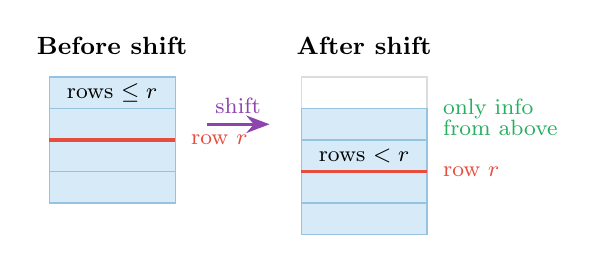
\begin{tikzpicture}[scale=0.4]
  % Before shift
  \node[font=\small\bfseries] at (2, 1) {Before shift};
  \foreach \r in {0,...,3}{
    \fill[lightblue, draw=cblue!50] (0, -\r) rectangle ++(4,-1);
  }
  \node[font=\footnotesize] at (2, -0.5) {rows $\leq r$};
  \draw[cred, very thick] (0, -2) -- (4, -2);
  \node[font=\footnotesize, cred, right] at (4.2, -2) {row $r$};

  % Arrow
  \draw[-{Stealth}, very thick, cpurple] (5, -1.5) -- (7, -1.5) node[midway, above, font=\footnotesize] {shift};

  % After shift
  \node[font=\small\bfseries] at (10, 1) {After shift};
  \fill[white, draw=cgray!30] (8, 0) rectangle ++(4,-1);
  \foreach \r in {1,...,3}{
    \fill[lightblue, draw=cblue!50] (8, -\r) rectangle ++(4,-1);
  }
  \fill[lightblue, draw=cblue!50] (8, -4) rectangle ++(4,-1);
  \node[font=\footnotesize] at (10, -2.5) {rows $< r$};
  \draw[cred, very thick] (8, -3) -- (12, -3);
  \node[font=\footnotesize, cred, right] at (12.2, -3) {row $r$};
  \node[font=\footnotesize, cgreen, right] at (12.2, -1) {only info};
  \node[font=\footnotesize, cgreen, right] at (12.2, -1.6) {from above};
\end{tikzpicture}

\vspace{0.3cm}
After shift: position $(r,c)$ in $v$ only contains information from rows \textbf{strictly above} $r$. \\
$\Rightarrow$ Autoregressive property preserved!
\end{columns}
\end{frame}

% ============================================================
\begin{frame}{Horizontal Stack + Vertical Connection}
\begin{columns}[c]
\column{0.45\textwidth}
\centering
\textbf{Horizontal Mask} ($1 \times 5$)\\[0.3cm]
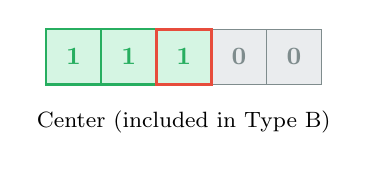
\begin{tikzpicture}[scale=0.7]
  \foreach \c in {0,...,4}{
    \ifnum\c<3
      \fill[lightgreen, draw=cgreen, thick] (\c, 0) rectangle ++(1,-1);
      \node[font=\small\bfseries, cgreen] at (\c+0.5, -0.5) {1};
    \else
      \fill[lightgray, draw=cgray] (\c, 0) rectangle ++(1,-1);
      \node[font=\small\bfseries, cgray] at (\c+0.5, -0.5) {0};
    \fi
  }
  \draw[cred, very thick] (2,0) rectangle ++(1,-1);
  \node[font=\footnotesize, below] at (2.5, -1.3) {Center (included in Type B)};
\end{tikzpicture}

\vspace{0.5cm}
Only sees \textbf{current row}, pixels to the \textbf{left} (and self for Type B).

\column{0.52\textwidth}
\textbf{Per-layer computation:}

\vspace{0.3cm}
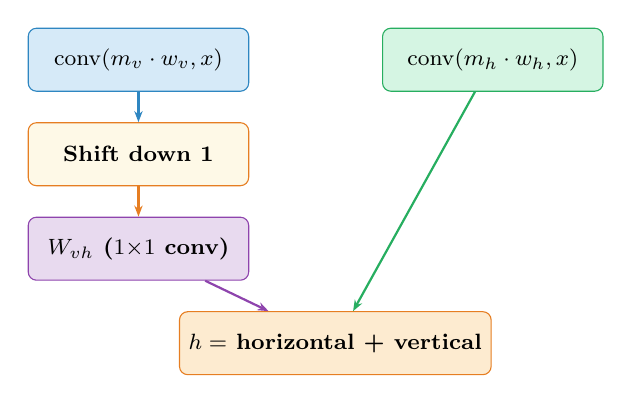
\begin{tikzpicture}[
  box/.style={draw, rounded corners=3pt, minimum width=2.8cm, minimum height=0.8cm, align=center, font=\footnotesize\bfseries},
  arr/.style={-{Stealth[length=4pt]}, thick}
]
  \node[box, fill=lightblue, draw=cblue] (vconv) at (0, 2) {$\mathrm{conv}(m_v \cdot w_v, x)$};
  \node[box, fill=lightyellow, draw=corange] (shift) at (0, 0.8) {Shift down 1};
  \node[box, fill=lightpurple, draw=cpurple] (w1) at (0, -0.4) {$W_{vh}$ ($1{\times}1$ conv)};

  \node[box, fill=lightgreen, draw=cgreen] (hconv) at (4.5, 2) {$\mathrm{conv}(m_h \cdot w_h, x)$};

  \node[box, fill=lightorange, draw=corange] (plus) at (2.5, -1.6) {$h = $ horizontal + vertical};

  \draw[arr, cblue] (vconv) -- (shift);
  \draw[arr, corange] (shift) -- (w1);
  \draw[arr, cpurple] (w1) -- (plus);
  \draw[arr, cgreen] (hconv) -- (plus);
\end{tikzpicture}

\vspace{0.3cm}
\[
  \boxed{h = \mathrm{conv}(m_h \cdot w_h, \; x) + W_{vh} \cdot v_{\text{shifted}}}
\]

\vspace{0.2cm}
The $1 \times 1$ conv merges vertical (above) and horizontal (left) information.
\end{columns}
\end{frame}

% ============================================================
\begin{frame}{How Upper-Right Info Reaches $\star$}
\centering
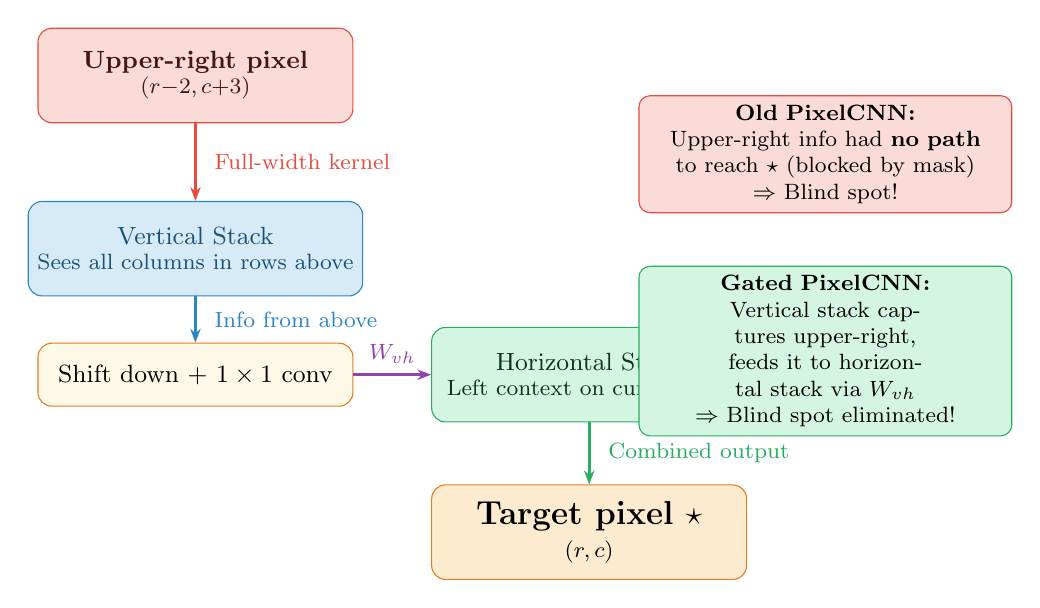
\begin{tikzpicture}[
  box/.style={draw, rounded corners=5pt, minimum width=4cm, minimum height=1.2cm, align=center, font=\small},
  arr/.style={-{Stealth[length=5pt]}, very thick}
]

  % Source pixel
  \node[box, fill=lightred, draw=cred, text=cred!30!black, font=\small\bfseries] (src) at (0, 4)
    {Upper-right pixel\\[-2pt]\footnotesize $(r{-}2, c{+}3)$};

  % Vertical stack
  \node[box, fill=lightblue, draw=cblue, text=darkblue] (vs) at (0, 1.8)
    {Vertical Stack\\[-2pt]\footnotesize Sees all columns in rows above};

  % Shift
  \node[box, fill=lightyellow, draw=corange, minimum height=0.8cm] (sh) at (0, 0.2)
    {Shift down + $1 \times 1$ conv};

  % Horizontal stack
  \node[box, fill=lightgreen, draw=cgreen, text=cgreen!30!black] (hs) at (5, 0.2)
    {Horizontal Stack\\[-2pt]\footnotesize Left context on current row};

  % Target
  \node[box, fill=lightorange, draw=corange, font=\large\bfseries] (tgt) at (5, -1.8)
    {Target pixel $\star$\\[-2pt]\footnotesize $(r, c)$};

  % Arrows
  \draw[arr, cred] (src) -- (vs) node[midway, right=3pt, font=\footnotesize] {Full-width kernel};
  \draw[arr, cblue] (vs) -- (sh) node[midway, right=3pt, font=\footnotesize] {Info from above};
  \draw[arr, cpurple] (sh) -- (hs) node[midway, above, font=\footnotesize] {$W_{vh}$};
  \draw[arr, cgreen] (hs) -- (tgt) node[midway, right=3pt, font=\footnotesize] {Combined output};

  % Old path (crossed out)
  \node[draw=cred, fill=lightred, rounded corners, text width=4.5cm, align=center, font=\footnotesize]
    at (8, 3) {
      \textbf{Old PixelCNN:}\\
      Upper-right info had \textbf{no path}\\
      to reach $\star$ (blocked by mask)\\
      $\Rightarrow$ Blind spot!
    };

  % New path (checkmark)
  \node[draw=cgreen, fill=lightgreen, rounded corners, text width=4.5cm, align=center, font=\footnotesize]
    at (8, 0.5) {
      \textbf{Gated PixelCNN:}\\
      Vertical stack captures upper-right,\\
      feeds it to horizontal stack via $W_{vh}$\\
      $\Rightarrow$ Blind spot eliminated!
    };

\end{tikzpicture}
\end{frame}

% ============================================================
\begin{frame}{Why Autoregressive Property is Preserved}

Three guarantees ensure pixel $(r, c)$ never sees itself or future pixels:

\vspace{0.4cm}
\begin{columns}[t]
\column{0.3\textwidth}
\centering
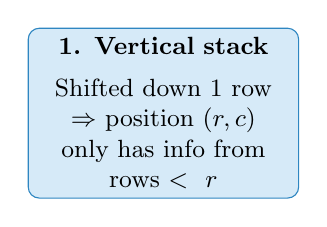
\begin{tikzpicture}
  \node[draw=cblue, fill=lightblue, rounded corners, minimum height=2cm, text width=3.2cm, align=center, font=\small] {
    \textbf{1. Vertical stack}\\[4pt]
    Shifted down 1 row\\
    $\Rightarrow$ position $(r,c)$\\only has info from\\rows $< r$
  };
\end{tikzpicture}

\column{0.3\textwidth}
\centering
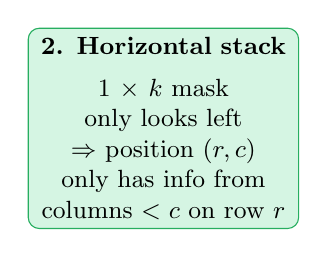
\begin{tikzpicture}
  \node[draw=cgreen, fill=lightgreen, rounded corners, minimum height=2cm, text width=3.2cm, align=center, font=\small] {
    \textbf{2. Horizontal stack}\\[4pt]
    $1 \times k$ mask\\only looks left\\
    $\Rightarrow$ position $(r,c)$\\only has info from\\columns $< c$ on row $r$
  };
\end{tikzpicture}

\column{0.3\textwidth}
\centering
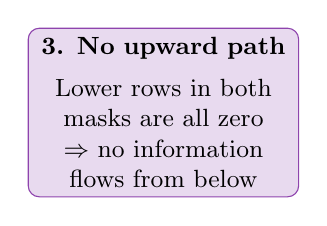
\begin{tikzpicture}
  \node[draw=cpurple, fill=lightpurple, rounded corners, minimum height=2cm, text width=3.2cm, align=center, font=\small] {
    \textbf{3. No upward path}\\[4pt]
    Lower rows in both\\masks are all zero\\
    $\Rightarrow$ no information\\flows from below
  };
\end{tikzpicture}
\end{columns}

\vspace{0.5cm}
\centering
Combined: $\star$ at $(r,c)$ only depends on pixels at $(r', c')$ where $r' < r$, or $r' = r$ and $c' < c$.\\[4pt]
This is exactly the \textbf{raster scan autoregressive ordering}.
\end{frame}

% ============================================================
\section{Summary}
% ============================================================

\begin{frame}{Summary: PixelCNN $\to$ Gated PixelCNN}

\renewcommand{\arraystretch}{1.6}
\centering
\begin{tabular}{p{3cm} p{4.5cm} p{4.5cm}}
\toprule
& \textbf{PixelCNN} & \textbf{Gated PixelCNN} \\
\midrule
\textbf{Structure} & Single masked conv per layer & Vertical + Horizontal stacks \\
\textbf{Mask shape} & $k \times k$, upper-left only & Vertical: $k \times k$ upper rows\newline Horizontal: $1 \times k$ left only \\
\textbf{Receptive field} & Sawtooth-shaped,\newline has \alert{blind spot} & Full coverage of all previous pixels \\
\textbf{Key trick} & --- & Shift down + $1 \times 1$ conv connects stacks \\
\textbf{Autoregressive} & Yes (by mask) & Yes (by mask + shift) \\
\bottomrule
\end{tabular}

\vspace{0.5cm}
\begin{block}{Key Takeaway}
The blind spot is caused by the \textbf{asymmetric information flow} in masked convolutions (full-width above, left-only on current row). Gated PixelCNN fixes this by \textbf{decoupling vertical and horizontal processing} and connecting them with a shifted $1 \times 1$ convolution.
\end{block}
\end{frame}

% ============================================================
\begin{frame}{}
\centering
\vspace{2cm}
{\Huge\bfseries Thank You}

\vspace{1cm}
{\large Questions?}
\end{frame}

\end{document}
